\documentclass[
t, % align text inside frame to t=top, b=bottom, c=center
10pt, % 8pt, 9pt, 10pt, 11pt, 12pt, 14pt, 17pt, 20pt available as text font
aspectratio=1610, % select your aspect ratio 4:3=43, 16:9=169, 16:10=1610
ngerman,
english,
%handout,
]{beamer}
\usetheme{Juelich}

\usepackage{babel}
\usepackage[utf8]{inputenc}

\title{Cognitive Computational Neuroscience}
\subtitle{Kriegeskorte \& Douglas (2018) Nature Neuroscience}
\author{Journal Club~~\vrule width0.3pt~~Julia Sprenger}
\institute[My Institute]{INM-6}
\date{\today}
\titlegraphic{
\includegraphics[height=0.8\paperheight]{material/drawing}}

\begin{document}
% only use \maketitle to set your titlepage
\fzjset{title page=image}
\maketitle

\part{Introduction}
% \makepart

\begin{frame}[label=history]
	\frametitle{Historical Background}
	\onslide<1->{
	Cognitive psychology
	\begin{itemize}
	 \item study of mental processes such as 'attention, language use, memory, perception, problem solving, creativity, and thinking'\footnote{\url{https://en.wikipedia.org/wiki/Cognitive_psychology}}\newline
	\end{itemize}
	}
	
	\onslide<2->{
	Allen Newell (1973)
	\begin{itemize}
	  \item 'You can't play 20 questions with nature and win'
	  \item Hypothesis testing needs to be complemented by the construction of comprehensive task-performing computational models\newline
% 	  \item tutorial is not complete yet, will be updated shortly
	\end{itemize}
	}
	
	\onslide<3->{
	Richard Feynman (1988)
	\begin{itemize}
	 \item 'What I cannot create, I do not understand'\newline
	\end{itemize}
    }
    
    \onslide<4->{
    \textbf{Cognitive Science (1980)}\\
    introduction of task-performing computational models (symbolic cognitive architectures, neural networks based on behavioural data)
    }
%     \onslide<4->{
%     \textbf{New Cognitive Neuroscience}\\
%     will be based on task-performing computational models, that explain how cognition arises from neurobiologically plausible dynamic components
%     }
\end{frame}

\begin{frame}
    \frametitle{Historical Background}
    Cognitive Neuroscience
    \begin{itemize}
     \item relate cognitive theories to the (human) brain using functional brain imaging
     \item mapping of cognitive functions to brain regions using
     \begin{itemize}
        \item EEG (1875)
        \item MEG (1968)
        \item PET (1950s)
        \item fMRI (1990)
     \end{itemize}
    \end{itemize}

\end{frame}

\begin{frame}
    \frametitle{Modern Imaging Techniques}
    \centering
    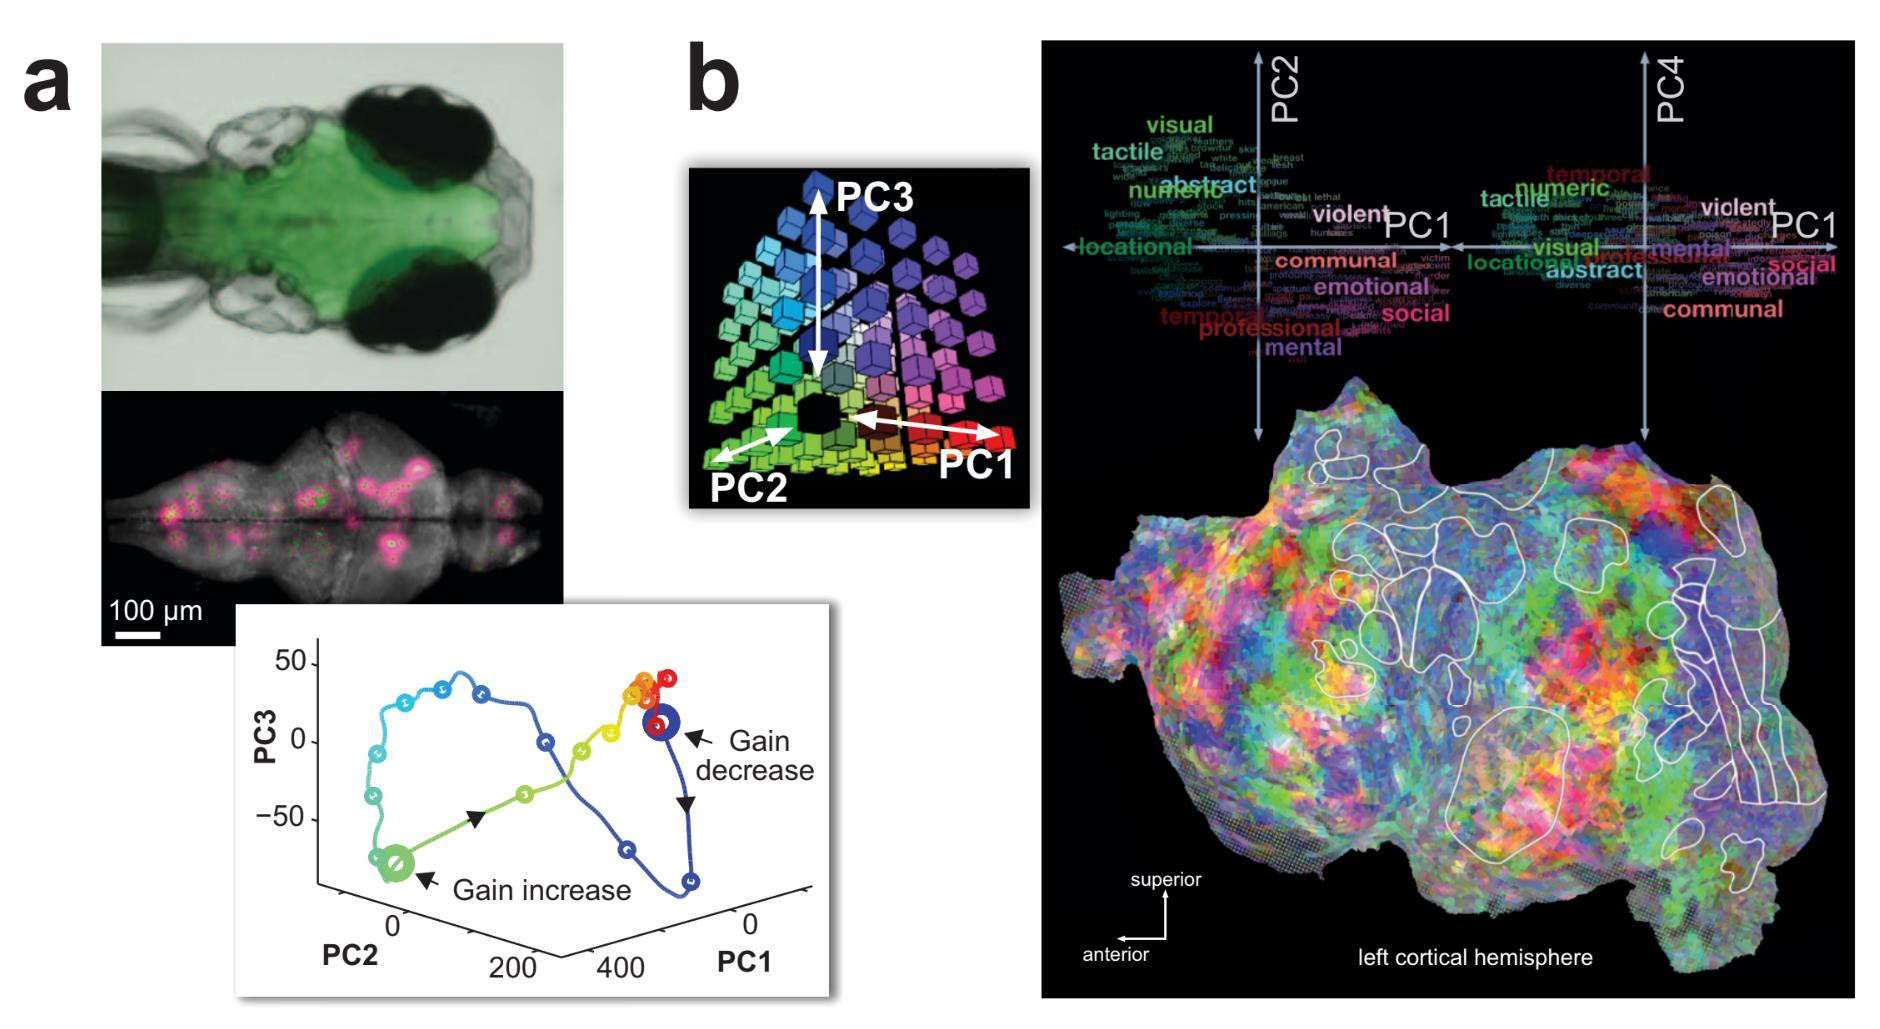
\includegraphics[height=0.7\textheight]{figures/figure1}
    \begin{itemize}
     \item a brain map does not reveal the computational mechanism
     \item but constrains for theory
     \item data-driven analysis provides only limited insights
    \end{itemize}

\end{frame}

\begin{frame}
    \frametitle{Advances in Cognitive Science}
    \begin{itemize}
     \item face-selective regions in human
     \item spacial clustering of face neurons in non-human primates
    \end{itemize}
\end{frame}


\begin{frame}[label=Approaches]
	\frametitle{Different Approaches}
	\onslide<1->{
	Cognitive sciences
	\begin{itemize}
	 \item interdisciplinary, scientific study of the mind and its processes\footnote{\url{https://en.wikipedia.org/wiki/Cognitive_sciencey}}
	 \item how humans learn \& think
	 \newline
	\end{itemize}
	}
	
	\onslide<2->{
	Computational Neuroscience
	\begin{itemize}
	  \item how brains adapt and compute\newline
	\end{itemize}
	}
	
	\onslide<3->{
	Artificial Intelligence
	\begin{itemize}
	 \item how to generate intelligent behaviour
	\end{itemize}
    }
\end{frame}


\begin{frame}
    \frametitle{Disciplines}
    \centering
    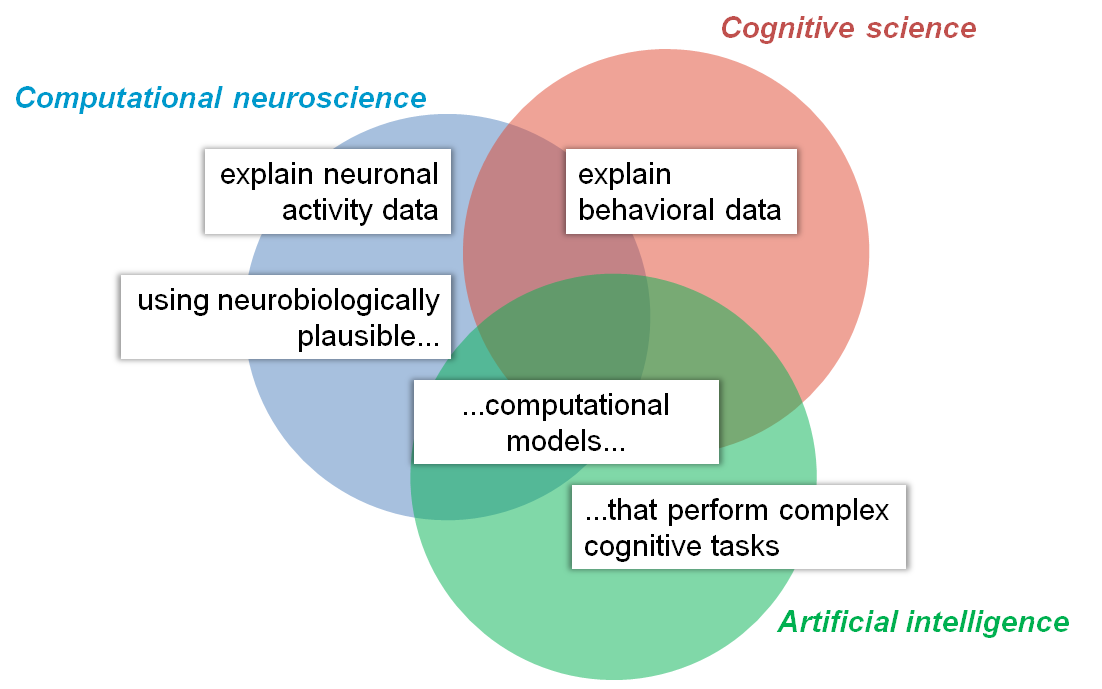
\includegraphics[height=0.7\textheight]{figures/figure2}
\end{frame}

\begin{frame}
    \frametitle{Recent advances}
    Cognitive Science
    \begin{itemize}
     \item top-down approach
     \item Bayesian cognitive models (optimal combination of prior knowledge with sensory evidence)
     \item unified perspective on probabilistic empirical inference
    \end{itemize}
    Computational Neuroscience
    \begin{itemize}
     \item bottom-up approach
     \item mathematical models of elementary computational components and their implementation with biological neurons
    \end{itemize}
    Artificial Intelligence
    \begin{itemize}
     \item demonstrates how component functions can be combined to create intelligent behaviour
     \item machine learning, deep neural networks
    \end{itemize}
    
    \textbf{Overarching Challenge}
    build solid bridges between theory and experiment
\end{frame}

\begin{frame}
    \frametitle{From Experiment Toward Theory}
    \begin{itemize}
     \item Models of connectivity and dynamics
     \item Decoding models
     \item Representational models
    \end{itemize}
\end{frame}

\begin{frame}
    \frametitle{The many meaning of model}
    \begin{itemize}
     \item Data-analysis models (statistical description of measured variables)
     \item box-and-arrow models (information processing)
     \item oracle model (relies on information without describing the extraction from input)
     \item brain-computational model (mimics brain information processing, eg sensory encoding)
     \item ...
    \end{itemize}

\end{frame}



\begin{frame}
    \frametitle{The Space of Process Models}
    \centering
    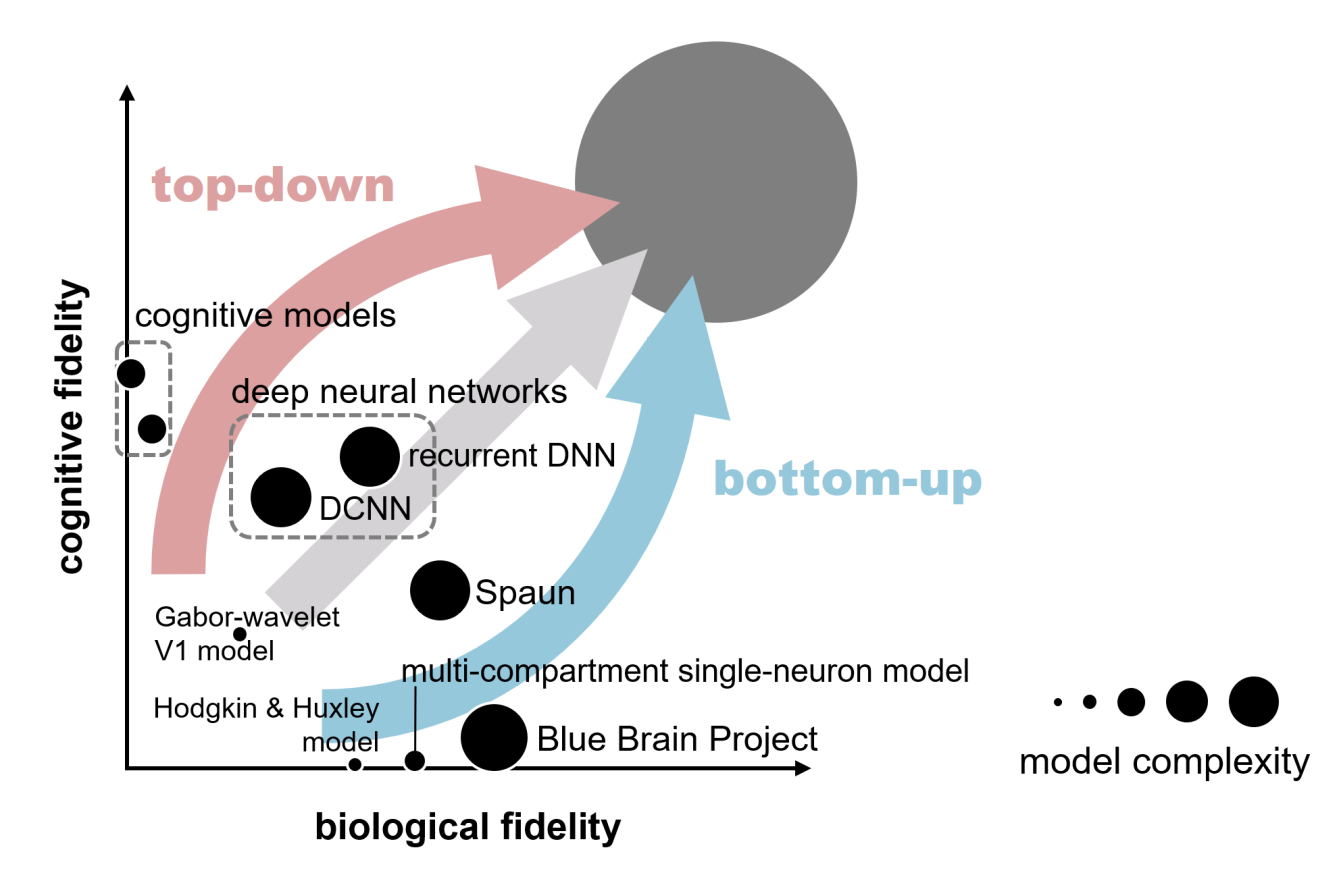
\includegraphics[height=0.7\textheight]{figures/figure3}
\end{frame}

\begin{frame}
    \frametitle{Interaction Among Sharable Components}
    \centering
    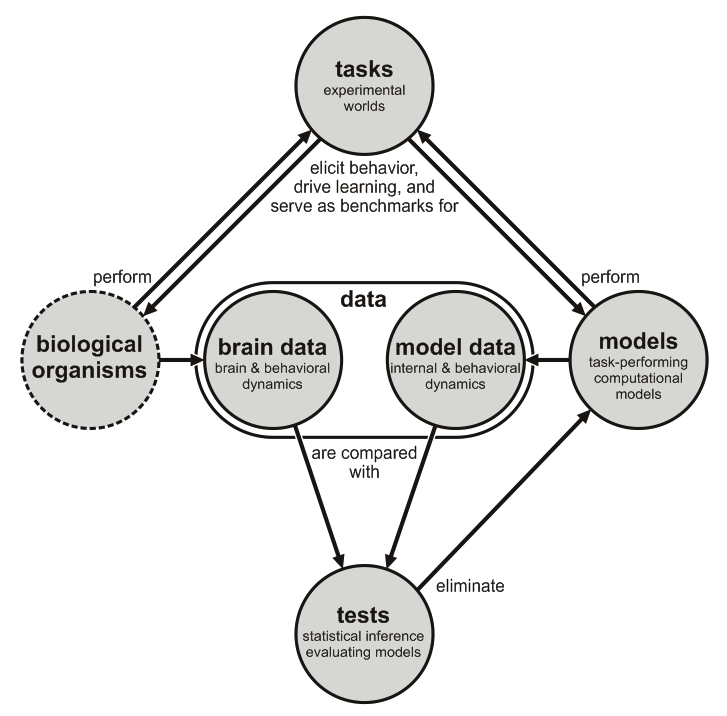
\includegraphics[height=0.7\textheight]{figures/figure4}
\end{frame}

% \begin{frame}[label=introduction]
% 	\frametitle{Motivation}
% 	\onslide<1->{
% 	Cognitive psychology
% 	\begin{itemize}
% 	 \item study of mental processes such as 'attention, language use, memory, perception, problem solving, creativity, and thinking'\footnote{\url{https://en.wikipedia.org/wiki/Cognitive_psychology}}\newline
% 	\end{itemize}
% 	}
% 	
% 	\onslide<2->{
% 	Allen Newell (1973)
% 	\begin{itemize}
% 	  \item 'You can't play 20 questions with nature and win'
% 	  \item Hypothesis testing needs to be complemented by the construction of comprehensive task-performing computational models\newline
% 	  \item tutorial is not complete yet, will be updated shortly
% 	\end{itemize}
% 	}
% 	
% 	\onslide<3->{
% 	Richard Feynman (1988)
% 	\begin{itemize}
% 	 \item 'What I cannot create, I do not understand'
% 	\end{itemize}
%     }
% \end{frame}

% \part{Installation}
% \makepart
% 
% \section{File Content}
% \begin{frame}[fragile]
% 	\frametitle{beamertheme-juelich.zip}
% 	The .zip archive consists of 1 directory with 3 subdirectories.
% 	\begin{itemize}
%       \item \verb+beamertheme-juelich.zip+
%       \item \verb+beamertheme-juelich/+ \hfill main directory of the .zip file
%       \begin{itemize}
%         \item \verb+sty/+ \hfill directory containing the .sty files
%         \begin{itemize}
%           \item \verb+fzj.pdf+ \hfill Juelich logo for pdf\LaTeX
%           \item \verb+beamerthemeJuelich.sty+ \hfill main style file
%           \item \verb+beamerouterthemeJuelich.sty+ \hfill aux. style file
%           \item \verb+beamerinnerthemeJuelich.sty+ \hfill aux. style file
%           \item \verb+beamerfontthemeJuelich.sty+ \hfill aux. style file
%           \item \verb+beamercolorthemeJuelich.sty+ \hfill aux. style file
%         \end{itemize}
%         \item[]
%         \item \verb+minimal/+ \hfill directory containing a minimal examples
%         \item[] 
%         \item \verb+tutorial/+ \hfill directory containing the sources to this tutorial
%       \end{itemize}
%     \end{itemize}
% \end{frame}
% 
% \section{Installation}
% \subsection{On Linux-based Machines}
% \begin{frame}[fragile]
% 	\frametitle{Linux Installation}
% 	\framesubtitle{Choose {\tt texmf} Tree}
% 	First, choose your favorite install directory.	\newline
% 	Then, create a new subdirectory \verb+beamertheme-juelich+
% 	\begin{block}{Change to your {\tt texmf} tree and create subdirectory}
%     \begin{itemize}
%       \item \verb+cd /usr/share/texmf/tex/latex/+ \hfill or
%       \item \verb+cd /usr/local/share/texmf/tex/latex/+ \hfill or
%       \item \verb+cd $HOME/texmf/tex/latex/+
%       \item \verb+mkdir beamertheme-juelich+
%     \end{itemize}
%     \end{block}
% \end{frame}
% 
% \begin{frame}[fragile]
% 	\frametitle{Linux: Install the {\tt .sty} Files}
% 	\begin{block}{Create Directory + Copy files + Update \TeX}
%     	\begin{itemize}
%           	\item Unzip \verb+beamertheme-juelich.zip+ file
%       		\item Copy all files from subdirectory \verb+beamertheme-juelich/sty+ into
%       		the new subdirectory \verb+beamertheme-juelich+
%       		\item[] 
%       		\item Try to compile the minimal example in the \verb+minimal+ subdirectory slide)
%       		\item Try to compile this tutorial in the \verb+tutorial+ subdirectory
%      	\end{itemize}
%     \end{block}
% \end{frame}
% 
% \section{Test Installation I}
% \begin{frame}[fragile,label=examples]
% 	\frametitle{Test your Installation}
% 	\framesubtitle{Try to compile this minimal talk}
% 	\begin{columns}
% 	\begin{column}[T]{0.4\textwidth}
% 	\footnotesize
% 	\begin{verbatim}
%      \documentclass{beamer}
%      \usetheme{Juelich}
% 
%      \title{My first talk with \LaTeX{}}
%      \subtitle{The template works!}
%      \author{Your Name}
%      \institute{Your Institute}
%      \date{\today}
%      \titlegraphic{\includegraphics%
%      [height=0.45\paperheight]{placeholder}
%      }
%      \begin{document}
%      \maketitle
%      \end{document}
% 	\end{verbatim}
% 	\end{column}\hfill
% 	\begin{column}[T]{0.4\textwidth}
% 	
\includegraphics[width=\textwidth]{minimal}
% 	\end{column}
% 	\end{columns}
% \end{frame}
% 
% \begin{frame}[fragile]
% 	\frametitle{Test your Installation II}
% 	\framesubtitle{Try to compile this minimal talk with handouts}
% 	\begin{columns}
% 	\begin{column}[T]{0.4\textwidth}
% 	\tiny
%  	\begin{verbatim}
%       \documentclass[t,handout]{beamer}
%       \usetheme{Juelich}
% 
%       \title{My first talk with \LaTeX{}}
%       \subtitle{The template works!}
%       \author{Your Name}
%       \institute{Your Institute}
%       \date{\today}
%       \titlegraphic{\includegraphics%
%       [height=0.45\paperheight]{placeholder}
%       }
%       \begin{document}
%       \maketitle
% 
%       \begin{frame}
%         \frametitle{My first slide title}
%         \framesubtitle{My first slide subtitle}
%       \ end{frame}
%       \end{document}
%  	\end{verbatim}
% 	\end{column}
% 	\begin{column}[T]{0.4\textwidth}
% 	
\includegraphics[height=0.7\textheight]{minimal_handout}
% 	\end{column}
% 	\end{columns}
% \end{frame}
% 
% \part{Examples}
% \makepart
% \section{Features}
% \selectlanguage{english}
% \frame{
% 	\frametitle{\LaTeX{}-Beamer Features}
% 	The following slides show how {\tt Latex-Beamer} constructs work within the
% 	template.
% 	\begin{itemize}
%       \item Framebreaks
%       \item Lists, numbered lists
%       \item Plain slides, background images
%       \item Theorems, proofs
%       \item Definitions, examples
%       \item Blocks, alert blocks
%       \item Highlight options
%       \item Formulae
%       \item Verbatim environments
%     \end{itemize}
% }
% 
% \section{Lists}
% \begin{frame}
% 	\frametitle{Lots of lists}
% 	\framesubtitle{Another Subtitle}
% 	\begin{itemize}
% 	  \item using the \texttt{pause} command:
% 	  \begin{itemize}
% 	    \item First item.
% 	    \pause
% 	    \item Second item.
% 	  \end{itemize}
% 	  \item using overlay specifications:
% 	  \begin{enumerate}
% 	    \item<3-> First numbered item.
% 	    \item<4-> Second numbered item.
% 	    \begin{itemize}
% 	      \item 3rd level item!
% 	    \end{itemize}
% 	  \end{enumerate}
% 	  \item using the general \texttt{uncover} command:
% 	  \begin{itemize}
% 	    \uncover<5->{\item First item.}
% 	    \uncover<6->{\item Second item.}
% 	  \end{itemize}
% 	\end{itemize}
% \end{frame}
% 
% \begin{frame}[fragile]
% 	\frametitle{Plain Frames}
% 	\begin{itemize}
%       \item The next slide shows a plain frame, even without the ``Jülich'' color
% 			bars at the left-hand side.
%       \item To use plain frames add the \verb![plain]! parameter to your \verb!\begin{frame}! statement.
%     \end{itemize}
% 	\begin{block}{How to use plain frames}
%     \tiny
% 	\begin{verbatim}
%     \begin{frame}[plain]
%     \frametitle{Plain Frame}
%       \begin{center}
%         Here is my tiny text on a plain frame.
%       \end{center} 
%     \ end{frame}
%     \end{verbatim}
% 	\end{block}
% \end{frame}
% 
% \begin{frame}[c,plain]
% 	\frametitle{Plain Frame}
% 	\begin{center}
% 		{\tiny Enough} {\scriptsize space} for {\Large your} {\huge big} {\Huge ideas.} {\TINY (or holiday pictures)}
% 	\end{center}
% \end{frame}
% 
% \section{Beamer Block Constructs}
% \subsection{Theorem, Proof}
% \begin{frame}
% 	\frametitle{Block Constructs}
% 	\framesubtitle{{\tt theorem, proof}}
% 	\begin{theorem}
% 	There is no largest prime number.
% 	\end{theorem}
% 	
% 	\begin{proof}
% 		\begin{enumerate}
% 			\item<1-| alert@1> Suppose $p$ were the largest prime number.
% 			\item<2-> Let $q$ be the product of the first $p$ numbers.
% 			\item<3-> Then $q+1$ is not divisible by any of them.
% 			\item<1-> Thus $q+1$ is also prime and greater than $p$.\qedhere
% 		\end{enumerate}
% 	\end{proof}
% \end{frame}
% 
% \subsection{Definition, Example}
% \begin{frame}
% 	\frametitle{Block Constructs}
% 	\framesubtitle{{\tt definition, example}}
% 	\begin{definition}
% 		A \alert{prime number} is a number that has exactly two divisors.
% 	\end{definition}
% 	\begin{example}
% 		\begin{itemize}
% 			\item 2 is prime (two divisors: 1 and 2).
% 			\item 3 is prime (two divisors: 1 and 3).
% 			\item 4 is not prime (\alert{three} divisors: 1, 2, and 4).
% 		\end{itemize}
% 	\end{example}
% \end{frame}
% 
% \subsection{Block, Alert Block}
% \begin{frame}
% 	\frametitle{Block Constructs}
% 	\framesubtitle{{\tt block, alertblock}}
% 	\begin{block}{Simple Block}
% 		Just some text.
% 	\end{block}
% 	\begin{alertblock}{Alert Block}
% 		This block seems to be pretty important.
% 	\end{alertblock}
% \end{frame}
% 
% \section{Highlight important information}
% \begin{frame}[fragile]
% 	\frametitle{Highlight important information}
% 	\framesubtitle{Use ``Jülich'' colors to attract attention }
% 	\begin{block}{Use {\tt \textbackslash{}emph\{\}}}
% 		\verb+This text is \emph{important}.+ \\
% 		This text is \emph{important}.  
% 	\end{block}
% 	\begin{block}{Use {\tt \textbackslash{}alert\{\}}}
% 		\verb+This text is \alert{really} important!+ \\
% 		This text is \alert{really} important!
% 	\end{block}
% \end{frame}
% 
% \section{Math Environment}
% \begin{frame}
% 	\frametitle{Math Environment}
% 	\framesubtitle{Use your {\LaTeX} formulae inside your slides without hassle}
% 	\[
% 	    \iiint\limits_V \operatorname{div} \vec{F} \, dV 
% 	    = \iint\limits_S \vec{F}\cdot d\vec{S}
% 	\]
% 	\[
% 	 \prod_{k=1}^n k = n! \,,\quad \sum_{k=1}^n k=\frac{n(n+1)}{2}\,,
% 	  \quad \int_0^{2\pi}\sin t\,dt=0
% 	\]
% 	\[
% 	    p(x)=\sum_{i=0}^n f_{i}q_{i}(x) \quad\mbox{with}\quad
% 	    q_{i}(x)=\prod_{\substack{k=0 \\ k\neq i}}^n
% 	    \frac{x-x_{k}}{x_{i}-x_{k}}\,.
% 	\]
% 	\[
% 	    \iint\limits_S (U \operatorname{grad} W)\cdot d\vec{S} 
% 	    =\iiint\limits_V (\operatorname{grad} U\cdot 
% 	     \operatorname{grad} W +U\Delta W)\,dV
% 	\]
% \end{frame}
% 
% \section{Code Environment}
% \begin{frame}[fragile]
% 	\frametitle{Verbatim Environment}
% 	\framesubtitle{Code Snippets}
% 	\begin{itemize}
%       \item Slides containing \verb!\verb! statements must be defined \verb+fragile+
%     \end{itemize}
%     	\tiny
%     	\begin{verbatim}
%  		\begin{frame}[fragile]
%         \frametitle{Hello World in Intercal}
%         \begin{verbatim}
%           DO ,1 <- #13
%           PLEASE DO ,1 SUB #1 <- #234
%           DO ,1 SUB #2 <- #112
%           DO ,1 SUB #3 <- #112
%           DO ,1 SUB #4 <- #0
%           DO ,1 SUB #5 <- #64
%           DO ,1 SUB #6 <- #194
%           DO ,1 SUB #7 <- #48
%           PLEASE DO ,1 SUB #8 <- #22
%           DO ,1 SUB #9 <- #248
%           DO ,1 SUB #10 <- #168
%           DO ,1 SUB #11 <- #24
%           DO ,1 SUB #12 <- #16
%           DO ,1 SUB #13 <- #214
%           PLEASE READ OUT ,1
%           PLEASE GIVE UP
%          \Xend{verbatim}                         % remove X after copy & paste :-)
%  		\ end{frame}
%  	    \end{verbatim}
% \end{frame}
% 
% \part{Jülich Colors}
% \makepart
% 
% \begin{frame}[label=colors]
%   \frametitle{Corporate Colors}
%   \framesubtitle{You can use predefined colornames to spice up your slides}
%   \centering
%   \begin{tikzpicture}
%     \foreach \color [count=\i] in {fzjblue, fzjlightblue, fzjred, fzjgreen, fzjyellow, fzjviolet, fzjorange} {
%       \node[fill=\color,circle,minimum size=2cm] at (\i*360/7: 2cm) {\color};
%     }
%   \end{tikzpicture}
% \end{frame}
% 
% \part{Localization}
% \makepart
% \section{Change Language}
% \begin{frame}[fragile,label=localization]
% 	\frametitle{Localization}
% 	\framesubtitle{How to change the date display to another language}
% 	The date will be adjusted automatically. You just have to use the {\tt babel}
% 	package with the desired language.
% 	\begin{block}{Date style -- Mixed}
% 		load package with DE and EN (default): \hfill \verb+\usepackage[ngerman,english]{babel}+ \newline
% 		choose German: \hfill \verb+\selectlanguage{ngerman}+ \newline
% 		choose English: \hfill \verb+\selectlanguage{english}+
% 	\end{block}	
% 	\begin{block}{Date style -- German}
% 		01. Januar 2018 \hfill
% 		\verb+\selectlanguage{ngerman}+
% 	\end{block}
% 	\begin{block}{Date style -- English}
% 		January 01, 2018 \hfill
% 		\verb+\selectlanguage{english}+
% 	\end{block}
% 
% \end{frame}
% 
% \selectlanguage{ngerman}
% \begin{frame}[fragile,,label=translation]
% 	\frametitle{Localization/Language}
% 	\framesubtitle{Change Helmholtz Banner Text}
% 	Using the \texttt{babel} package with the language option automatically sets
% 	the correct labels for the slide counter and Helmholtz banner.
% 	
% 	\begin{block}{Helmholtz Banner and Date in German}
% 	\begin{itemize}
% 	  \item Take a look at the date and Helmholtz banner in the lower left
% 	  corner and the slide name adn frame number in the middle
% 	  \item This slide should show the german version
% 	  \item Enable options via \verb+\documentclass[english,ngerman]{beamer}+
% 	  \item Enabled locally via \verb+\selectlanguage{ngerman}+ before
% 	  \verb+\begin{frame}+
% 	\end{itemize}
% 	\end{block}
% \end{frame}
% 
% \selectlanguage{english}
% \author{Your Name}
% \part{Tweaks}
% \makepart
% \section{Slide Number Display}
% 
% \begin{frame}[fragile,label=tweaks]
% 	\frametitle{Slide Number Display}
% 	\framesubtitle{How to change the slide number style}
% 	\begin{block}{Full Display: Current Slide | Overall Number of Slides}
% 		\scriptsize\verb+\setbeamertemplate{frame number}[full]+ \hfill 
% 		\scriptsize\usebeamercolor[fg]{frametitle} Slide 42 $|$ 524
% 	\end{block}
% 	\begin{block}{No Display: empty}
% 		\scriptsize\verb+\setbeamertemplate{frame number}[empty]+ \hfill
% 		\scriptsize\usebeamercolor[fg]{frametitle}
% 	\end{block}
% 	\begin{block}{Default Display: Current Slide}
% 		\scriptsize\verb+\setbeamertemplate{frame number}[default]+ \hfill 
% 		\scriptsize\usebeamercolor[fg]{frametitle} Slide 42
% 	\end{block}
% 	\begin{block}{Translation}
% 	If you choose german as language the name \emph{Slide} will be translated
% 	to \emph{Folie} automatically (See \hyperlink{translation}{\alert{this}}
% 	slide)
% 	\end{block}
% \end{frame}
% 
% \section{Partner Logos}
% 
% \setbeamertemplate{footer element1}[logo]{jara}%
% \setbeamertemplate{footer element3}[logo]{uni_bonn}%
% \setbeamertemplate{footer element2}[logo]{rwth}%
% 
% \begin{frame}[fragile]
% 	\frametitle{Project Partners}
% 	\framesubtitle{How to set up partner logos}
% 	\begin{itemize}
%       \item Show up to 3 partner logos, on this slide Jara, RWTH, Bonn
%       \item Design your logos with sufficiently large white borders
%       \item {pdf\LaTeX} pictures file types: \verb+.pdf .png .jpg+
%     \end{itemize}
% 	\begin{block}{Show logos}
%     	\verb+\setbeamertemplate{footer element1}[logo]{jara}+
% 		\verb+\setbeamertemplate{footer element2}[logo]{uni_bonn}+
%         \verb+\setbeamertemplate{footer element3}[logo]{rwth}+
%     \end{block}
% 	\begin{block}{Reset back to default settings}
%     	\verb+\setbeamertemplate{footer element1}[default]+
%     	\verb+\setbeamertemplate{footer element1}[default]+
%     	\verb+\setbeamertemplate{footer element1}[default]+    	
%     \end{block}
% \end{frame}
% \setbeamertemplate{footer element1}[default]
% \setbeamertemplate{footer element2}[default]
% \setbeamertemplate{footer element3}[default]
% 
% \part{Handouts}
% \makepart
% \section{Handouts}
% \begin{frame}[fragile,label=handouts,t]
% 	\frametitle{Create Handouts}
% 	\begin{block}{Switch and Setup Render Mode}
%      \scriptsize
%      		\verb+\documentclass[handout]{beamer}+\\
% 			\verb+\mode<handout>{+\\
% 			\verb+\pgfpagesuselayout{4 on 1}[a4paper,landscape,border shrink=5mm]}+
%     \end{block}
% 	\begin{block}{Define Number of Pages per Sheet}
%     	\scriptsize
%     	\verb+\pgfpagesuselayout{2 on 1}[a4paper,border shrink=5mm]+
%     	\verb+\pgfpagesuselayout{4 on 1}[a4paper,landscape,border shrink=5mm, landscape]+
%     	\verb+\pgfpagesuselayout{8 on 1}[a4paper,border shrink=5mm]+
%     	\verb+\pgfpagesuselayout{16 on 1}[a4paper,landscape,border shrink=5mm, landscape]+
%     \end{block}
% 	\begin{block}{Further Reading -- See {\tt Latex-Beamer} manual for details}
%     	{\tiny
%     	{\tt www.ctan.org/tex-archive/macros/latex/contrib/beamer/doc/beameruserguide.pdf}}
%     \end{block}
% \end{frame}
% 
% \part{Aspect Ratio}
% \begin{frame}[fragile]
% 	\frametitle{Aspect Ratio}
% 	The documentclass allows several ratios for the slide. Just change the variable \verb+aspectratio+.
% 	\begin{itemize}
% 	  \item \verb+aspectratio=43+ gives classical 4:3 ratio
% 	  \item \verb+aspectratio=169+ gives classical 16:9 ratio
% 	  \item \verb+aspectratio=1610+ gives classical 16:10 ratio
% 	\end{itemize}
% \end{frame}
% 
% \part{Style}
% \begin{frame}[fragile]
% 	\frametitle{Style}
% 	The design allows two styles.
% 	\begin{block}{Style with Image}
% 	\begin{itemize}
% 	\item for the title page: \verb+\fzjset{title page=image}+
% 	\item for the part page: \verb+\fzjset{section page=image}+
%     \item for the section page: \verb+\fzjset{section page=image}+
%     \end{itemize}
% 	\end{block}
% 	
% 	\begin{block}{Style with Text}
%     \begin{itemize}
% 	\item for the title page: \verb+\fzjset{title page=text}+
% 	\item for the part page: \verb+\fzjset{section page=text}+
%     \item for the section page: \verb+\fzjset{section page=text}+
%     \end{itemize}
% 	\end{block}
% \end{frame}
% 
% \begin{frame}[fragile]
%     \frametitle{Allcaps or Regular Title Fonts}
%     It is possible to switch the style of the font via the options
%     \begin{itemize}
%       \item \verb+\fzjset{title=allcaps}+ to set the title in allcaps
%       \item \verb+\fzjset{title=regular}+ to set the title regular
%       \item \verb+\fzjset{subtitle=allcaps}+ to set the title in allcaps for short text
%       \item \verb+\fzjset{subtitle=regular}+ to set the title regular and in a smaller font for long text
%       \item \verb+\fzjset{part=allcaps}+ to set the part in allcaps for short text
%       \item \verb+\fzjset{part=regular}+ to set the part regular and in a smaller font for long text    
%     \end{itemize}
% \end{frame}
% 
% \fzjset{title=regular}
% \fzjset{title page=text}
% \subtitle{Now in text only mode and regular text}
% \maketitle
% 
% \fzjset{title page=image}
% \subtitle{Now back in image mode}
% \maketitle
% 
% \part{This is a part page}
% \fzjset{part page=text}
% \makepart
% 
% \section{This is a section page}
% \fzjset{section page=text}
% \subtitle{This is a section page}
% \makesection
% 
% \section{Bugs}
% \begin{frame}[fragile,label=bugs]
% 	\frametitle{Fixed Bugs}
% 	\begin{block}{Nothing reported yet.}
% 	~
%     \end{block}
% 	\begin{block}{More Pitfalls/bugs?}
% 	 	Please report.
%     \end{block}
% \end{frame}
% 
% 
% \part{Extensions}
% \makepart
% \begin{frame}[fragile]
% 	\frametitle{Poster with \LaTeX -Beamer}
% 	To create scientific posters with {\LaTeX} the \verb!beamerposter! extension
% 	can be used. Template will be provided soon.
% 	\begin{block}{More Information at}
%     \small
%     \url{http://www-i6.informatik.rwth-aachen.de/~dreuw/latexbeamerposter.php}
%     \end{block}
% \end{frame}
% 
% \part{Contact Information}
% \begin{frame}[c,label=contact]
% 	\frametitle{Contact}
% 	\begin{center}
% 		\Large \emph{Thank you for using this template!}
% 	\end{center}
% 	\begin{block}{Enhance Missing Functionality Yourself!}
% 		Please send your enhancements along with a short description to {\tt i.kabadshow@fz-juelich.de}
% 	\end{block}
% 	\begin{block}{Report Problems}
% 		Please report problems with the template or uncommon behavior to {\tt i.kabadshow@fz-juelich.de}
% 	\end{block}
% \end{frame}

\end{document}
